%!TEX root = ../../main.tex
\chapter{The Nonlinear Surface Susceptibility}\label{chap:chi2}
\partialtoc


In this chapter we formulate a theoretical approach of surface second-harmonic
generation from semiconductor surfaces based on the length gauge and the
electron density operator. Within the independent particle approximation the
nonlinear second-order surface susceptibility tensor
$\chi^{\mathrm{a}\mathrm{b}\mathrm{c}}(-2\omega;\omega,\omega)$ is calculated,
including in one unique formulation (i) the scissors correction, needed to have
the correct value of the energy band gap, (ii) the contribution of the nonlocal
part of the pseudopotentials, routinely  used in \textit{ab initio} band
structure calculations, and (iii) the derivation for the inclusion of the cut
function, used to extract the surface response. The first two contributions are
described by spatially nonlocal quantum mechanical operators and are fully taken
into account in the present formulation.


%%%%%%%%%%%%%%%%%%%%%%%%%%%%%%%%%%%%%%%%%%%%%%%%%%%%%%%%%%%%%%%%%%%%%%%%%%%%%%%%
%%%%%%%%%%%%%%%%%%%%%%%%%%%%%%%%%%%%%%%%%%%%%%%%%%%%%%%%%%%%%%%%%%%%%%%%%%%%%%%%

\section{The Nonlinear Surface Susceptibility}

In this section I will outline the general procedure to obtain the surface
susceptibility tensor for SHG. We start with the nonlinear polarization
$\mathbf{P}(\mathbf{r})$ of a bulk system, written as
\begin{equation}\label{mshg}
\begin{split}
P^{\mathrm{a}}(\mathbf{r},2\omega)
= \chi^{\mathrm{abc}}(-2\omega;\omega,\omega)
  E^{\mathrm{b}}(\mathbf{r},\omega)E^{\mathrm{c}}(\mathbf{r},\omega)
+ \chi^{\mathrm{abcd}}(-2\omega;\omega,\omega)
  E^{\mathrm{b}}(\mathbf{r},\omega)\nabla^{\mathrm{c}}
  E^{\mathrm{d}}(\mathbf{r},\omega)
+ \cdots,
\end{split}
\end{equation}
where $\chi^{\mathrm{abc}}(-2\omega;\omega,\omega)$ and
$\chi^{\mathrm{abcd}}(-2\omega;\omega,\omega)$ correspond to the dipolar and
quadrupolar susceptibility tensors, and $\mathbf{E}(\mathbf{r})$ is the incoming
electric field along the different Cartesian directions denoted by the roman
superscripts. For ease of notation, I will drop the $\omega$ arguments from this
point on. At this point I introduce the units of the quantities above. For
simplicity, we use the MKS system of units. The units of
$\mathbf{E}(\mathbf{r})$ are $[\mathbf{E}] = $ V/m, and the units of
$\mathbf{P}(\mathbf{r})$ are $[\mathbf{P}] = $ V/m since
$\mathbf{P}(\mathbf{r})$ is a \emph{bulk} polarization. Therefore, the units of
the bulk $\chi^{\mathrm{abc}}$ are $[\chi^{\mathrm{abc}}] = $ m/V.

If we consider a semi-infinite system with a centrosymmetric bulk, we can obtain
a bulk and a surface nonlinear polarization that differ from each other from
symmetry considerations alone. To show this, we take
\begin{equation}\label{mshg2}
P^{\mathrm{a}}(\mathbf{r})
= \chi^{\mathrm{abc}}E^{\mathrm{b}}(\mathbf{r})E^{\mathrm{c}}(\mathbf{r})
+ \chi^{\mathrm{abcd}}E^{\mathrm{b}}(\mathbf{r})
  \frac{\partial}{\partial\mathbf{r}^{\mathrm{c}}}E^{\mathrm{d}}(\mathbf{r}) 
+ \cdots,
\end{equation}
as the polarization with respect to the $\mathbf{r}$ coordinate system, and 
\begin{equation}\label{mshg3}
P^{\mathrm{a}}(-\mathbf{r})
= \chi^{\mathrm{abc}}E^{\mathrm{b}}(-\mathbf{r})E^{\mathrm{c}}(-\mathbf{r})
+ \chi^{\mathrm{abcd}}E^{\mathrm{b}}(-\mathbf{r})
  \frac{\partial}{\partial(-\mathbf{r}^{\mathrm{c}})}E^{\mathrm{d}}(-\mathbf{r}) 
+ \cdots, 
\end{equation}
as the polarization in the inverted coordinate system, where we take
$\mathbf{r}$ to $-\mathbf{r}$. Note that we have kept the same susceptibility
tensors as they must be invariant under $\mathbf{r} \to -\mathbf{r}$ since the
system is centrosymmetric. Recalling that $\mathbf{P}(\mathbf{r})$ and
$\mathbf{E}(\mathbf{r})$ are polar vectors
\cite{jacksonbook}, we have that Eq. \eqref{mshg3} reduces to
\begin{align}\label{mshg4}
-P^{\mathrm{a}}(\mathbf{r})
&= \chi^{\mathrm{abc}}(-E^{\mathrm{b}}(\mathbf{r}))(-E^{\mathrm{c}}(\mathbf{r}))
 + \chi^{\mathrm{abcd}}(-E^{\mathrm{b}}(\mathbf{r}))
(-\frac{\partial}{\partial\mathbf{r}^{\mathrm{c}}})(-E^{\mathrm{d}}(\mathbf{r})) 
 + \cdots,\nonumber\\
P^{\mathrm{a}}(\mathbf{r})
&= -\chi^{\mathrm{abc}}E^{\mathrm{b}}(\mathbf{r})E^{\mathrm{c}}(\mathbf{r})
 + \chi^{\mathrm{abcd}}E^{\mathrm{b}}(\mathbf{r})
   \frac{\partial}{\partial\mathbf{r}^{\mathrm{c}}}E^{\mathrm{d}}(\mathbf{r}) 
 + \cdots,
\end{align}
that when compared with Eq. \eqref{mshg2} leads to the conclusion that
\begin{equation}\label{sshg}
\begin{split}
\chi^{\mathrm{abc}} &= 0,\\
&\qquad\qquad\text{(centrosymmetric bulk)}\\
\chi^{\mathrm{abcd}} &\ne 0,
\end{split}
\end{equation}
for a centrosymmetric bulk.

The surface of a centrosymmetric system necessarily breaks the centrosymmetry;
thus, there are no symmetry restrictions imposed on the $\chi^{\mathrm{abc}}$
produced from the surface region. Therefore, it is convenient to define the
surface nonlinear polarization $\mathbf{P}_{\mathrm{surface}}$ as follows,
\begin{equation}\label{sshgp}
P^{\mathrm{a}}_{\mathrm{surface}}
\equiv \chi^{\mathrm{abc}}_{\mathrm{surface}}E^{\mathrm{b}}E^{\mathrm{c}},
\end{equation}
where $\chi^{\mathrm{abc}}_{\mathrm{surface}}$ is the surface nonlinear
susceptibility. In this case, the MKS units of $[\mathbf{P}_{\mathrm{surface}}]$
are V, and $[\chi^{\mathrm{abc}}_{\mathrm{surface}}]$ are m$^{2}$/V. The
contribution from $\chi^{\mathrm{abcd}}$ to the surface polarization is
neglected as it originates from a higher order multipole. From Eq. \eqref{mshg}
we have that for the bulk of a semi-infinite system,
\begin{equation}\label{sshgp3}
P^{\mathrm{a}}_{\mathrm{bulk}}
= \chi^{\mathrm{abcd}}_{\mathrm{bulk}}
  E^{\mathrm{b}}\nabla^{\mathrm{c}}E^{\mathrm{d}},  
\end{equation}
which is the bulk nonlinear polarization; in this case the dipolar contribution
$\chi^{\mathrm{abc}}_{\mathrm{bulk}} = 0$ since we are in the centrosymmetric
bulk. As it follows from Ref. \cite{bloembergenPR62}, the surface nonlinear
polarization is of dipolar electric order while the bulk polarization is of
quadrupolar electric and dipolar magnetic order. The surface
$\boldsymbol{\chi}_{\mathrm{surface}}$ and bulk
$\boldsymbol{\chi}_{\mathrm{bulk}}$ susceptibilities are tensors of rank
three and four, respectively.

In this work, we will only concentrate on SSHG, even though bulk-generated SH is
also a very important optical phenomenon. To this end, we will neglect the
contribution from Eq. \eqref{sshgp3} and only consider the surface term from Eq.
\eqref{sshgp}. I will also exclude other interesting surface SH phenomena like,
electric field induced second-harmonic (EFISH), which would be represented by a
surface susceptibility tensor of quadrupolar origin. As mentioned in Chapter
\ref{chap:intro}, in centrosymmetric systems for which the quadrupolar bulk
response is much smaller than the dipolar surface response, SH is a very capable
and powerful optical surface probe \cite{downerSIA01}.

In the following sections of this chapter, we show the theoretical
approach to derive the expressions for the surface susceptibility tensor
$\chi^{\mathrm{abc}}_{\mathrm{surface}}$.

\begin{figure}[t]
\centering
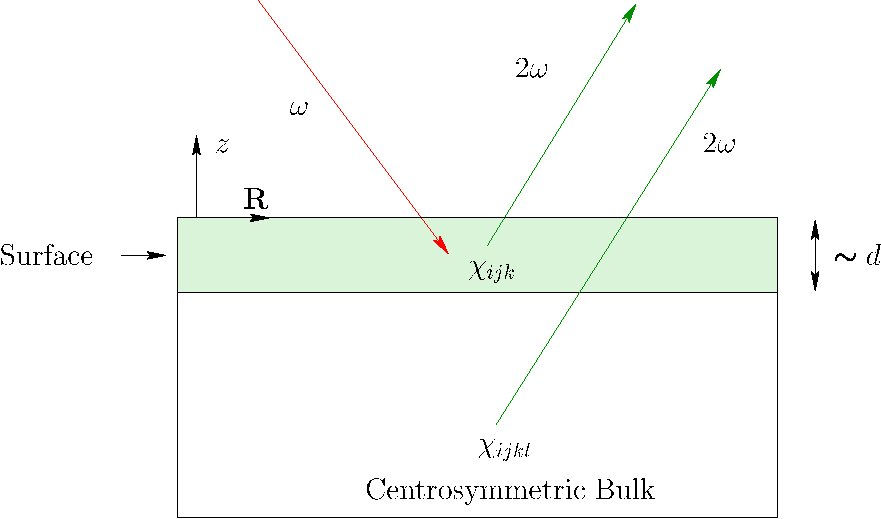
\includegraphics[scale=0.6]{content/figures/diag-system}
\caption{Sketch of a semi-infinite system with a centrosymmetric bulk. The
surface region is of width $\sim d$. The incoming photon of frequency $\omega$
is represented by a downward red arrow, whereas both the surface and bulk
created second-harmonic photons of frequency $2\omega$ are represented by upward
green arrows. The red color suggests an incoming infrared photon with a green
second-harmonic photon. The dipolar ($\chi^{\mathrm{abc}}_{\mathrm{surface}}$),
and quadrupolar ($\chi^{\mathrm{abcd}}_{\mathrm{bulk}}$) susceptibility tensors
are shown in the regions where they are nonzero. The $z$-axis is perpendicular
to the surface and $\mathbf{R}$ is parallel to it.}
\label{fsystem}
\end{figure}


%%%%%%%%%%%%%%%%%%%%%%%%%%%%%%%%%%%%%%%%%%%%%%%%%%%%%%%%%%%%%%%%%%%%%%%%%%%%%%%%
%%%%%%%%%%%%%%%%%%%%%%%%%%%%%%%%%%%%%%%%%%%%%%%%%%%%%%%%%%%%%%%%%%%%%%%%%%%%%%%%

\section{Time-dependent Perturbation Theory}\label{tdpt}

We assume the IPA, a classical electromagnetic field, and quantum mechanical
matter. We neglect local field and excitonic effects. We can describe the system
using the one electron density operator ${\rho}$, with which we can calculate
the expectation value of a single-particle observable $\mathcal{O}$ as
\begin{equation}\label{traza}
\left\langle\mathcal{O}\right\rangle
= \mathrm{Tr}(\rho\mathcal{O}),
\end{equation}
with $\mathcal{O}$ the associated quantum mechanical operator and Tr the 
trace. The density operator satisfies
\begin{equation}\label{eqrho}
i\hbar \frac{d\rho}{dt} = \left[H,\rho\right],
\end{equation}
with $H(t)$ as the total single electron Hamiltonian, written as 
\begin{equation*}
H(t) = H_{0} + H_{I}(t),  
\label{achea}
\end{equation*}
where $H_{0}$ is the unperturbed time-independent Hamiltonian, and $H_{I}(t)$ is
the time-dependent potential energy due to the interaction of the electron with
the electromagnetic field. To proceed with the solution of $\rho$ it is
convenient to use the interaction picture, where a unitary operator
\begin{equation}\label{ou}
U = e^{iH_{0}t/\hbar},
\end{equation}
transforms any operator $\mathcal{O}$ into
\begin{equation}\label{ip}
\tilde{\mathcal{O}} = U\mathcal{O}U^{\dagger}.
\end{equation}
Even if $\mathcal{O}$ is time-independent, $\tilde{\mathcal{O}}$ is
time-dependent through the explicit time dependence of $U$. The dynamical
equation for $\tilde{\rho}$ is given by
\begin{equation}\label{intrho}
i\hbar \frac{d\tilde{\rho}}{dt}
= \left[-e\mathbf{r}(t)\cdot\mathbf{E}(t),\tilde{\rho}\right]
= [\tilde{H}_{I}(t), \tilde{\rho}],
\end{equation}
with solution 
\begin{equation}\label{intrho2}
i\hbar \tilde{\rho}(t)
= i\hbar \tilde{\rho}_{0} + 
\int_{-\infty}^{t}
\left[\tilde{H}_{I}(t^{\prime}),\tilde{\rho}(t^{\prime})\right]\,dt^{\prime},  
% \label{trans}
\end{equation}
where $\tilde{\rho}_{0} = \tilde{\rho}(t = -\infty)$ is the unperturbed density
matrix.

We assume that the interaction is switched-on adiabatically and choose a
time-periodic perturbing field, to write
\begin{equation}\label{efield}
\mathbf{E}(t)
= \mathbf{E} e^{-i\omega t}e^{\eta t}
= \mathbf{E} e^{-i\tilde{\omega} t},
\end{equation}
with
\begin{equation}\label{got}
\tilde{\omega} =\omega + i\eta,
\end{equation} 
where $\eta > 0$ assures that at $t = -\infty$, the interaction is zero and has
its full strength $\mathbf{E}$ at $t = 0$. After computing the required time
integrals one takes $\eta\to 0$. Also, $\tilde{\rho}(t = -\infty)$ should be
time independent and thus $[\tilde{H}_{I},\tilde{\rho}]_{t = -\infty} = 0$. This
implies that $\tilde{\rho}(t = -\infty)\equiv\tilde{\rho}_{0}$, such that
\begin{equation}\label{nrhon}
\langle n\mathbf{k}\vert \tilde{\rho}_{0} \vert m\mathbf{k}'\rangle
= f_{n}(\hbar\omega^{\Sigma}_{n}(\mathbf{k}))
\delta_{nm}\delta(\mathbf{k}-\mathbf{k}'),
\end{equation}
with $f_{n}(\hbar\omega^{\Sigma}_{n}(\mathbf{k})) = f_{n}$ as the Fermi-Dirac
distribution function. For a clean, cold semiconductor $f_{n}=1$ when $n$ is a
valence ($v$) or occupied band, and zero when $n$ is a conduction ($c$) or empty
band. We assume this for the remainder of this work. As we neglect spin-orbit
coupling, the final expression for $\chi^{\mathrm{abc}}(-2\omega;\omega,\omega)$
has to be multiplied by a factor of 2 to account for spin-degeneracy. The
expectation values must always satisfy $\langle\mathcal{O}\rangle =
\mathrm{Tr}({\rho}\mathcal{O}) = Tr(\tilde{\rho}\tilde{\mathcal{O}})$.

We solve Eq. \eqref{intrho2} using the standard iterative
solution, for which we write
\begin{equation}\label{rhop}
\tilde{\rho}
= \tilde{\rho}^{(0)}
+ \tilde{\rho}^{(1)}
+ \tilde{\rho}^{(2)}
+ \cdots,
\end{equation}
where $\tilde{\rho}^{(N)}$ where the superscript denotes the order (power) with
which each term depends on the perturbation $H_{I}(t)$. Then, Eq.
\eqref{intrho2} reads
\begin{equation}\label{intrho3}
  \tilde{\rho}^{(0)} 
+ \tilde{\rho}^{(1)} 
+ \tilde{\rho}^{(2)} 
+ \cdots
= \tilde{\rho}_{0}
+ \frac{1}{i\hbar}\int_{-\infty}^{t} 
  \left[
  \tilde{H}_{I}(t'),\tilde{\rho}^{(0)}+\tilde{\rho}^{(1)}+\tilde{\rho}^{(2)}
  + \cdots
  \right]\,dt',
\end{equation}
where, by equating equal orders in the perturbation, we find
\begin{equation}\label{rho0}
\tilde{\rho}^{(0)}\equiv\tilde{\rho}_{0},
\end{equation}
and the $N$th-order term
\begin{equation}\label{rhoN}
\tilde{\rho}^{(N)}(t)=
\frac{1}{i\hbar}
\int_{-\infty}^{t}
\left[\tilde{H}_{I}(t'),\tilde{\rho}^{(N-1)}(t')\right]\,dt'.
\end{equation}
It is simple to show that matrix elements of Eq. (\ref{rhoN}) satisfy 
$\langle n\mathbf{k}| \rho^{(N+1)}(t) |m\mathbf{k}'\rangle =
\rho^{(N+1)}_{nm}(\mathbf{k})\delta(\mathbf{k}-\mathbf{k}')$, with
\begin{equation}\label{rtilde}
\tilde{\rho}^{(N+1)}_{nm}(\mathbf{k};t)
= \frac{e}{i\hbar}\int_{-\infty}^t
\langle n\mathbf{k}|
\left[\mathbf{r}(t'),\tilde{\rho}^{(N)}(t')\right]
|m\mathbf{k}\rangle
\cdot\mathbf{E}(t')dt'.
\end{equation}
This shows that the $N + 1$ solution is determined by the $N$th solution, which
in turn is determined by the $N - 1$ solution, and so on. Starting from the
zeroth order solution given in Eq. \eqref{rho0}, we can solve Eq. \eqref{rtilde}
for any desired order.

We will look for the expectation value of the microscopic current density,
$\mathbf{J}$, given by
\begin{equation*}
\mathbf{J} = \langle{\mathbf{J}}\rangle 
           = \frac{e}{A}\mathrm{Tr}({\rho}\dot{\mathbf{r}}),
\end{equation*}
where $\dot{\mathbf{r}}$ is the time derivative of the position operator of the
electron with charge $e$, defined as
\begin{equation}
\mathbf{v}\equiv \dot{\mathbf{r}}=\frac{1}{i\hbar }[\mathbf{r},H_0],  
\label{mv}
\end{equation}
with $\mathbf{v}$ the velocity operator of the electron, and $A$ the area of the
unit cell. We calculate the polarization density $\mathbf{P}$, related to
$\mathbf{J}$ by $\mathbf{J}=d\mathbf{P}/dt$. We write the second-order nonlinear
polarization as,
\begin{equation}\label{pshg}
\boldsymbol{\mathcal{P}}^{\mathrm{a}}(2\omega)=
\chi^{\mathrm{abc}}_{\mathrm{surface}}(-2\omega;\omega,\omega)
E^{\mathrm{b}}(\omega)E^{\mathrm{c}}(\omega),  
\end{equation}
where $\chi^{\mathrm{a}\mathrm{b}\mathrm{c}}(-2\omega ;\omega ,\omega )$ is the
nonlinear susceptibility responsible for surface second-harmonic generation
(SSHG). The superscripts in Eq. \eqref{pshg} denote Cartesian components, and if
repeated are to be summed over. Without loss of generality we will define
$\chi^{\mathrm{abc}}_{\mathrm{surface}}(-2\omega;\omega,\omega)$ to satisfy
intrinsic permutation symmetry,
$\chi^{\mathrm{abc}}_{\mathrm{surface}}(-2\omega;\omega ,\omega )
=\chi^{\mathrm{acb}}_{\mathrm{surface}}(-2\omega ;\omega,\omega )$.

The unperturbed Hamiltonian is used to solve the Kohn-Sham equations
\cite{kohnPR65} of Density Functional Theory (DFT). It is convenient to work
within the Local Density Approximation (LDA), so we label the hamiltonian with
the corresponding LDA superscript. Any other approximation can be used (like the
generalized gradient approximation) and our derivation remains the same. Then,
\begin{equation}\label{ache.2}
H^{\mathrm{LDA}}_{0}(\mathbf{r},\mathbf{p})
= \frac{p^{2}}{2m_e}+V(\mathbf{r},\mathbf{p})
\end{equation}
with $m_e$ the mass of the electron, $\mathbf{p}=-i\hbar\boldsymbol{\nabla}$ its
canonical momentum, and $V$ the periodic crystal potential, where we neglect
spin-orbit terms. To be more general in our derivation of
$\chi^{\mathrm{abc}}(-2\omega;\omega,\omega)$, we assume
contribution as is customary for most pseudopotentials, and then we replace $V$
with
\begin{equation}
V^{\mathrm{ps}}(\mathbf{r},\mathbf{p})
= V(\mathbf{r})+V^{\mathrm{nl}}(\mathbf{r},\mathbf{p}),
\end{equation}
where $V(\mathbf{r})$ and $V^{\mathrm{nl}}(\mathbf{r},\mathbf{p})$ are the local
and nonlocal parts, respectively. The argument $(\mathbf{r},\mathbf{p})$ is
equivalent to the explicit $(\mathbf{r},\mathbf{r}')$ nonlocal notation
\cite{ismailPRL01}. For this nonlocal part, we have that
\begin{align}\label{ache.3n}
V^{\mathrm{nl}}(\mathbf{r},\mathbf{r}')\equiv
\langle\mathbf{r}\vert
V^{\mathrm{nl}}
\vert\mathbf{r}'\rangle \neq 0 
\quad\text{for}\quad\mathbf{r} \neq \mathbf{r}',
\end{align}
where $V^{\mathrm{nl}}(\mathbf{r},\mathbf{r}')$ is a function of $\mathbf{r}$
and $\mathbf{r}'$ representing the nonlocal contribution of the pseudopotential.
In case of a local potential, i.e. $V= V(\mathbf{r})$, like that of all-electron
schemes, we simply omit the contribution of
$V^{\mathrm{nl}}(\mathbf{r},\mathbf{p})$ from the results that we have derived.

It is well known that the use of the LDA leads to an underestimation of the band
gap. A standard procedure to correct for this is to use the ``scissors
approximation'', where the conduction bands are rigidly shifted in energy so
that the band gap corresponds to the accepted experimental electronic band
gap.\cite{levinePRL89,levinePRL91,delsolePRB93} This is often in fairly good
agreement with the GW band gap based on a more sophisticated
calculation.\cite{hybertsenPRB86} The LDA wave functions are used since they
produce band structures with dispersion relations similar to those predicted by
the GW. Mathematically, the scissors (non-local) operator $S$ is added to the
unperturbed or unscissored Hamiltonian $H^{\mathrm{LDA}}_{0}$ ,
\begin{equation}\label{ache.1}
H^\Sigma_{0}(\mathbf{r},\mathbf{p})
= H^{\mathrm{LDA}}_{0}(\mathbf{r},\mathbf{p})
+ S(\mathbf{r},\mathbf{p})
\end{equation}
where 
\begin{equation}\label{hats}
S(\mathbf{r},\mathbf{p}) = \hbar \Delta\sum_{n}\int (1-f_{n})
|n\mathbf{k}\rangle\langle n\mathbf{k}|\,d^{3}k,
\end{equation}
with $\hbar\Delta$ the rigid ($\mathbf{k}$-independent) energy correction to be
applied. The unscissored and scissored Hamiltonians satisfy
\begin{align*}
H^{\mathrm{LDA}}_{0}(\mathbf{r},\mathbf{p})\psi _{n\mathbf{k}}(\mathbf{r}) &=
\hbar \omega^{\mathrm{LDA}}_{n}(\mathbf{k})\psi _{n\mathbf{k}}(\mathbf{r}),
\label{hamils} \\\\
H_{0}^\Sigma (\mathbf{r},\mathbf{p})\psi _{n\mathbf{k}}(\mathbf{r}) &=
\hbar \omega_{n}^\Sigma(\mathbf{k})\psi _{n\mathbf{k}}(\mathbf{r}),
\end{align*}
where the scissor-shifted energies, $\omega_{n}^\Sigma(\mathbf{k})$, are given
by
\begin{equation}\label{chon.78}
\omega_{n}^\Sigma(\mathbf{k})
= \omega^\mathrm{LDA}_{n}(\mathbf{k})+(1-f_{n})\Delta.
\end{equation}
Lastly, the Schr\"odinger equation reads
\begin{align}\label{ache.4} 
\left(
\frac{-\hbar^2}{2m_{e}}\nabla^{2}
+ V(\mathbf{r})
\right)
\psi_{n\mathbf{k}}(\mathbf{r})
+ \int V^{\mathrm{nl}}(\mathbf{r},\mathbf{r}')
  \psi_{n\mathbf{k}}(\mathbf{r}')\,d\mathbf{r}'
= E_{i}\psi_{n\mathbf{k}}(\mathbf{r}),
\end{align} 
where $\psi_{n\mathbf{k}}(\mathbf{r}) = \langle\mathbf{r}|n\mathbf{k}\rangle =
e^{i\mathbf{k}\cdot\mathbf{r}}u_{n\mathbf{k}}(\mathbf{r})$, are the real space
representations of the Bloch states $|n\mathbf{k}\rangle$ labeled by the band
index $n$ and the crystal momentum $\mathbf{k}$, and
$u_{n\mathbf{k}}(\mathbf{r})$ is cell periodic. We emphasize that the scissored
and unscissored Hamiltonian have the same eigenfunctions.


%%%%%%%%%%%%%%%%%%%%%%%%%%%%%%%%%%%%%%%%%%%%%%%%%%%%%%%%%%%%%%%%%%%%%%%%%%%%%%%%
%%%%%%%%%%%%%%%%%%%%%%%%%%%%%%%%%%%%%%%%%%%%%%%%%%%%%%%%%%%%%%%%%%%%%%%%%%%%%%%%

\section{Length Gauge}\label{longi}

According to Ref. \cite{ismailPRL01}, we first start with the interaction
Hamiltonian expressed in the velocity gauge, containing the nonlocal parts
$V^{nl}(\mathbf{r},\mathbf{p})$ and $S (\mathbf{r},\mathbf{p})$. Within the
dipole approximation and using a gauge transformation, it can be transformed
into an effective Hamiltonian \cite{valerie}
\begin{equation}
H_{I}(t)=-e\mathbf{r}\cdot \mathbf{E}(t).
\label{rde}
\end{equation}
The treatment of the position operator $\mathbf{r}$ for extended Bloch states is
problematic and has been discussed in Refs. \cite{adamsJCP53, blountSSP62} and
will be dealt with in Appendix \ref{app:re_ri}. The matrix elements of
$\mathbf{r}$ are split between the \emph{intraband} ($\mathbf{r}_{i}$) and
\emph{interband} ($\mathbf{r}_{e}$) parts, where $\mathbf{r} = \mathbf{r}_{i} +
\mathbf{r}_{e}$ \cite{adamsJCP53, blountSSP62}, and its matrix elements are
\cite{aversaPRB95}
\begin{align}\label{rnminn}
\langle n\mathbf{k}\vert \mathbf{r}_{i} |m\mathbf{k}'\rangle 
&= \delta_{nm}
\left[
  \delta(\mathbf{k} - \mathbf{k}')\boldsymbol{\xi}_{nn}(\mathbf{k})
+ i\nabla_{\mathbf{k}}\delta(\mathbf{k} - \mathbf{k}')
\right],\\
\langle n\mathbf{k}| \mathbf{r}_{e} |m\mathbf{k}'\rangle 
&= (1- \delta_{nm})\delta(\mathbf{k}-\mathbf{k}')
   \boldsymbol{\xi}_{nm}(\mathbf{k}),\label{rnmenn}
\end{align}
such that $\mathbf{r}_{e,nm}=0$ for $n=m$, and
\begin{equation}\label{zetann}
\boldsymbol{\xi}_{nm}(\mathbf{k})
\equiv i\frac{(2\pi)^3}{\Omega}
\int_{\Omega}u^{*}_{n\mathbf{k}}(\mathbf{r})
\nabla_{\mathbf{k}}\,u_{m\mathbf{k}}(\mathbf{r})
\,d\mathbf{r},
\end{equation}
where $\Omega$ is the unit cell volume. The interband part, $\mathbf{r}_{e}$,
can be obtained as follows. We use $H^{\Sigma}_{0}$ in Eq. \eqref{mv} to obtain
the velocity operator
\begin{equation}\label{vop}
\mathbf{v}^{\Sigma}
= \frac{1}{i\hbar}
\left[\mathbf{r},H^{\Sigma}_{0}\right],
\end{equation}
and calculating its matrix elements
\begin{equation}\label{conhrnm}
i\hbar\langle n\mathbf{k}\vert\mathbf{v}^\Sigma\vert m\mathbf{k}\rangle
= \langle n\mathbf{k}\vert
  \left[\mathbf{r},H^{\Sigma}_{0}\right]
  \vert m\mathbf{k}\rangle
= \langle n\mathbf{k}\vert
  \mathbf{r}H^{\Sigma}_{0} - H^{\Sigma}_{0}\mathbf{r}
  \vert m\mathbf{k}\rangle
= \left(
  \hbar\omega^{\Sigma}_{m}(\mathbf{k}) - \hbar\omega^{\Sigma}_{n}(\mathbf{k})
  \right)
  \langle n\mathbf{k}\vert\mathbf{r}\vert m\mathbf{k}\rangle.
\end{equation}
Defining $\omega^\Sigma_{nm}(\mathbf{k}) =
\omega^{\Sigma}_{n}(\mathbf{k}) - \omega^\Sigma_m(\mathbf{k})$, we get
\begin{equation}\label{pmnrmn}
\mathbf{r}_{nm}(\mathbf{k})
= \frac{\mathbf{v}^\Sigma_{nm}(\mathbf{k})}{i\omega^\Sigma_{nm}(\mathbf{k})}
\qquad n\notin D_{m},
\end{equation} 
which can be identified as
$\mathbf{r}_{nm}=(1-\delta_{nm})\boldsymbol{\xi}_{nm}\to \mathbf{r}_{e,nm}$.
Here, $D_m$ are all the possible degenerate $m$-states.For the intraband part,
$\mathbf{r}_i$ only appears in commutators during the derivation of the optical
response. We use \cite{aversaPRB95}
\begin{equation}\label{conmri3n}
\langle n\mathbf{k}\vert
\left[\mathbf{r}_{i},\mathcal{O}\right]
\vert m\mathbf{k}'\rangle
= i\delta(\mathbf{k} - \mathbf{k}')(\mathcal{O}_{nm})_{;\mathbf{k}},
\end{equation}  
where
\begin{equation}\label{gendevnn}
(\mathcal{O}_{nm})_{;\mathbf{k}} =
  \nabla_{\mathbf{k}}\mathcal{O}_{nm}(\mathbf{k})
- i\mathcal{O}_{nm}(\mathbf{k})
\left(
\boldsymbol{\xi}_{nn}(\mathbf{k}) - \boldsymbol{\xi}_{mm}(\mathbf{k})
\right),
\end{equation} 
is the generalized derivative of the operator $\mathcal{O}$ (see Appendix
\ref{app:re_ri}). The vectors $\boldsymbol{\xi}_{nn}(\mathbf{k})$ are defined in 
Ref. \cite{aversaPRB95} though they do not need to be calculated explicitly in
what follows.

As can be seen from Eq. \eqref{ache.1} and \eqref{ache.2}, both $\mathcal{S}$
and $V^{\mathrm{nl}}$ are nonlocal potentials. Their contribution in the
calculation of the optical response must be considered in order to get reliable
results \cite{ismailPRL01}. Before continuing, we derive a key result for the
length gauge formulation. Then,
\begin{equation}\label{vop2}
\begin{split}
\mathbf{v}^{\Sigma}
&=\mathbf{v} + \mathbf{v}^{\mathrm{nl}} 
+ \mathbf{v}^{\mathcal{S}}
= \mathbf{v}^\mathrm{LDA} + \mathbf{v}^{\mathcal{S}}\\
&=\frac{\mathbf{p}}{m_{e}} + \frac{1}{i\hbar}
  \left[\mathbf{r},V^{\mathrm{nl}}(\mathbf{r},\mathbf{r}')\right]
+ \frac{1}{i\hbar}
  \left[\mathbf{r},\mathcal{S}(\mathbf{r},\mathbf{p})\right],
\end{split}
\end{equation}
where we have defined
\begin{equation}\label{conhr}
\begin{split}
\mathbf{v} &=\frac{\mathbf{p}}{m_{e}}\\
\mathbf{v}^{\mathrm{nl}} &= \frac{1}{i\hbar}
  \left[\mathbf{r},V^{\mathrm{nl}}\right]\\
\mathbf{v}^{\mathcal{S}} &= \frac{1}{i\hbar}
  \left[\mathbf{r},S(\mathbf{r},\mathbf{p})\right]\\
\mathbf{v}^\mathrm{LDA} &= \mathbf{v}+\mathbf{v}^{\mathrm{nl}}
\end{split}
\end{equation}  
$\mathbf{p}= -i\hbar\boldsymbol{\nabla}$ is the momentum operator, and
using $[r^a,p^b]=i\hbar\delta_{ab}$, where $\delta_{ab}$ is the Kronecker
delta. Using Eq. \eqref{hats}, we obtain that the matrix elements of
$\mathbf{v}^{\mathcal{S}}$ are given by
\begin{equation}\label{chon.2} 
\mathbf{v}^{\mathcal{S}}_{nm} = i\Delta f_{mn}\mathbf{r}_{nm},
\end{equation}
with $f_{nm} \equiv f_{n} - f_{m}$, where we see that
$\mathbf{v}^{\mathcal{S}}_{nn} = 0$. From Eqs. \eqref{pmnrmn} and \eqref{vop2}
it follows that
\begin{align}\label{chon.8}
\mathbf{v}^\Sigma_{nm} 
&= \mathbf{v}^\mathrm{LDA}_{nm} + i\Delta f_{mn}\mathbf{r}_{nm}\nonumber\\
&= \mathbf{v}^\mathrm{LDA}_{nm} + i\Delta f_{mn}
   \frac{\mathbf{v}^\Sigma_{nm}(\mathbf{k})}{i\omega^\Sigma_{nm}(\mathbf{k})}
   \nonumber\\
%%%%%%%%%%%%%%%%%%%%%%%%%%%%%%%%%%%%%%%%%%%%%%%%%
\mathbf{v}^\Sigma_{nm}
  \frac{\omega^\Sigma_{nm}-\Delta f_{mn}}{\omega^\Sigma_{nm}}
&= \mathbf{v}^\mathrm{LDA}_{nm}\nonumber\\
%%%%%%%%%%%%%%%%%%%%%%%%%%%%%%%%%%%%%%%%%%%%%%%%%
\mathbf{v}^\Sigma_{nm}\frac{\omega^{\mathrm{LDA}}_{nm}}{\omega^\Sigma_{nm}}
&= \mathbf{v}^\mathrm{LDA}_{nm}\nonumber\\
%%%%%%%%%%%%%%%%%%%%%%%%%%%%%%%%%%%%%%%%%%%%%%%%%
\frac{\mathbf{v}^\Sigma_{nm}}{\omega^\Sigma_{nm}}
&= \frac{\mathbf{v}^\mathrm{LDA}_{nm}}{\omega^{\mathrm{LDA}}_{nm}},
\end{align}
since $\omega^\Sigma_{nm}-\Delta f_{mn}=\omega^{\mathrm{LDA}}_{nm}$. Therefore,
\begin{align}\label{chon.9}
\begin{split}
\mathbf{v}^\Sigma_{nm}(\mathbf{k}) &=
\frac{\omega^\Sigma_{nm}}{\omega^{\mathrm{LDA}}_{nm}}
\mathbf{v}^\mathrm{LDA}_{nm}(\mathbf{k})
= \left(
1 + \frac{\Delta}{\omega_c(\mathbf{k})-\omega_v(\mathbf{k})}
\right)
\mathbf{v}^\mathrm{LDA}_{nm}(\mathbf{k})\qquad n\notin D_{m}\\\\
\mathbf{v}^\Sigma_{nn}(\mathbf{k}) &= \mathbf{v}^\mathrm{LDA}_{nn}(\mathbf{k}),
\end{split}
\end{align} 
and Eq. \eqref{pmnrmn} gives
\begin{align}\label{chon.10}
\mathbf{r}_{nm}(\mathbf{k})
= \frac{\mathbf{v}^\Sigma_{nm}(\mathbf{k})}{i\omega^\Sigma_{nm}(\mathbf{k})}
= \frac{\mathbf{v}^\mathrm{LDA}_{nm}(\mathbf{k})}
{i\omega^{\mathrm{LDA}}_{nm}(\mathbf{k})} \qquad n\notin D_{m}.
\end{align}
The matrix elements of $\mathbf{r}_{nm}(\mathbf{k})$ are identical using either
the LDA or scissored Hamiltonian, thus negating the need to label them. Of
course, it is more convenient to calculate them through
$\mathbf{v}^\mathrm{LDA}_{nm}(\mathbf{k})$ which includes only the contribution
of $\mathbf{v}^\mathrm{nl}_{nm}(\mathbf{k})$. These can be readily calculated
for fully separable nonlocal pseudopotentials in the Kleinman-Bylander
form.\cite{olevano, mottaCMS10, kleinmanPRL82, adolphPRB96} The advantage of
using the electron density operator along with the length gauge formalism for
calculating linear and nonlinear optical responses, for the scissored
Hamiltonian, resides in the ease with which the scissors operator can be
introduced into the calculation by simply using the unscissored LDA Hamiltonian,
$H_0^{\mathrm{LDA}}$, for the unperturbed system with $-e\mathbf{r}\cdot
\mathbf{E}(t)$ as the interaction. We stress that within the length gauge, we
need only replace $\omega^{\mathrm{LDA}}_{n}$ with $\omega_{n}^{\Sigma}$ at the
end of the derivation to obtain the scissored results for any susceptibility
expression, whether linear or nonlinear \cite{nastosPRB05}. In Appendix
\ref{app:vnlme} we outline how this is accomplished.

We also need to derive the matrix elements the density operator. In order to
proceed, we must now work out the commutator of Eq. \eqref{rtilde}. Then,
\begin{align}\label{conmu1}
\langle n\mathbf{k}|
\left[\mathbf{r}(t),\tilde{\rho}^{(N)}(t)\right]
|m\mathbf{k}\rangle
%%%%%%%%%%%%%%%%%%%%%%%%%%%%%%%%%%%%%%%%%%%%%%%%%%%%%%%%
&= \langle n\mathbf{k}|
\left[U\mathbf{r}U^\dagger,U\rho^{(N)}(t)U^\dagger\right]
|m\mathbf{k}\rangle\nonumber \\
%%%%%%%%%%%%%%%%%%%%%%%%%%%%%%%%%%%%%%%%%%%%%%%%%%%%%%%%
&= \langle n\mathbf{k}|
U\left[\mathbf{r},\rho^{(N)}(t)\right]U^\dagger
|m\mathbf{k}\rangle\\
%%%%%%%%%%%%%%%%%%%%%%%%%%%%%%%%%%%%%%%%%%%%%%%%%%%%%%%%
&= e^{i\omega^\Sigma_{nm}t}
\left(
\langle n\mathbf{k}|
  \left[\mathbf{r}_{e},\rho^{(N)}(t)\right]
+ \left[\mathbf{r}_{i},\rho^{(N)}(t)\right]
|m\mathbf{k}\rangle
\right)\nonumber,
\end{align}
where the time dependence of the operator in the interaction picture is
explicitly shown by the exponential factor, and the implicit dependence of
$\rho^{(N)}$ inherited from Eq. \eqref{eqrho} is given through the $t$ argument.
We calculate the interband term first, so using Eq. \eqref{chon.10} we obtain
\begin{align}\label{conmu2}
\langle n\mathbf{k}|
\left[\mathbf{r}_{e},\tilde{\rho}^{(N)}(t)\right]
|m\mathbf{k}\rangle
&= \sum_{q}
\left(
  \langle n\mathbf{k}| \mathbf{r}_{e} |q\mathbf{k}\rangle
  \langle q\mathbf{k}| \tilde{\rho}^{(N)}(t) |m\mathbf{k}\rangle
- \langle n\mathbf{k}| \tilde{\rho}^{(N)}(t) |q\mathbf{k}\rangle
  \langle q\mathbf{k}| \mathbf{r}_{e} |m\mathbf{k}\rangle
\right)\nonumber \\
&= \sum_{q\ne n,m}
\left(
  \mathbf{r}_{nq}(\mathbf{k})
  \rho^{(N)}_{q m}(\mathbf{k};t)
- \rho^{(N)}_{nq}(\mathbf{k};t)
  \mathbf{r}_{q m}(\mathbf{k})
\right)\nonumber\\
& \equiv \mathbf{R}^{(N)}_{e}(\mathbf{k};t),
\end{align}
and from Eq. \eqref{conmri3n},
\begin{equation}\label{conmri4}
\langle n\mathbf{k}|
[\mathbf{r}_i,\tilde{\rho}^{(N)}(t)]
|m\mathbf{k}'\rangle
=i \delta(\mathbf{k}-\mathbf{k}') (\rho^{(N)}_{nm}(t))_{;\mathbf{k}}
\equiv \delta(\mathbf{k}-\mathbf{k}')\mathbf{R}_i^{(N)}(\mathbf{k};t).
\end{equation}
Then Eq. \eqref{rtilde} becomes
\begin{equation}\label{rtilde2}
\tilde{\rho}^{(N+1)}_{nm}(\mathbf{k};t)
= \frac{ie}{\hbar}\int_{-\infty}^{t}
e^{i(\omega^{\Sigma}_{nm} - \tilde{\omega})t'}
\left[
  R_{e}^{\mathrm{b}(N)}(\mathbf{k};t')
+ R_{i}^{\mathrm{b}(N)}(\mathbf{k};t')
\right]
E^{\mathrm{b}}\,dt',
\end{equation}
where the roman superindices $\mathrm{abc}$ denote Cartesian components that are
summed over if repeated. Starting from the linear response and proceeding from
Eq. \eqref{nrhon} and  \eqref{conmu2},
\begin{align}\label{R0e}
R_e^{\mathrm{b}(0)}(\mathbf{k};t)
&=
\sum_{q}
\left(
r^{\mathrm{b}}_{nq}(\mathbf{k})
\rho^{(0)}_{q m}(\mathbf{k})
-
\rho^{(0)}_{nq}(\mathbf{k})
r^{\mathrm{b}}_{q m}(\mathbf{k})
\right)
\nonumber \\
&=
\sum_{q}
\left(
r^{\mathrm{b}}_{nq}(\mathbf{k})
\delta_{q m}f_m(\hbar\omega^\Sigma_m(\mathbf{k}))
-
\delta_{nq}f_n(\hbar\omega^{\Sigma}_{n}(\mathbf{k}))
r^{\mathrm{b}}_{q m}(\mathbf{k})
\right)
\nonumber \\
&= f_{mn}r^{\mathrm{b}}_{nm}(\mathbf{k}),
\end{align}
where $f_{mn} = f_{m}-f_{n}$. From now on, it should be clear that the matrix
elements of $\mathbf{r}_{nm}$ imply $n\notin D_m$. We also have from Eq.
\eqref{conmri4} and Eq. \eqref{gendevnn} that
\begin{equation}\label{R0i}
R_i^{\mathrm{b}(0)}(\mathbf{k})
= i(\rho^{(0)}_{nm})_{;k^{\mathrm{b}}}
= i\delta_{nm}(f_{n\mathbf{k}})_{;k^{\mathrm{b}}}
= i\delta_{nm}\nabla_{k^{\mathrm{b}}} f_{n\mathbf{k}}.
\end{equation}
For a semiconductor at $T = 0$, $f_{n} = 1$ if the state $|n\mathbf{k}\rangle$
is a valence state and $f_{n} = 0$ if it is a conduction state. Thus,
$\nabla_\mathbf{k} f_{n} = 0$, $\mathbf{R}_i^{(0)} = 0$ and the linear response
has no contribution from the intraband transitions. Then,
\begin{align}\label{rtilde2n}
\tilde{\rho}^{(1)}_{nm}(\mathbf{k};t)
&= \frac{ie}{\hbar} f_{mn}
   r^{\mathrm{b}}_{nm}(\mathbf{k})E^{\mathrm{b}}
   \int_{-\infty}^{t} dt'
   e^{i(\omega^\Sigma_{nm}-\tilde{\omega})t'}\nonumber \\
&= \frac{e}{\hbar}
f_{mn}
r^{\mathrm{b}}_{nm}(\mathbf{k})E^{\mathrm{b}}
\frac{e^{i(\omega^\Sigma_{nm}-\tilde{\omega})t}}
{\omega^\Sigma_{nm}-\tilde{\omega}}
\nonumber \\
&=
e^{i(\omega^\Sigma_{nm}-\tilde{\omega})t}
B^{\mathrm{b}}_{mn}(\mathbf{k})E^{\mathrm{b}}(t)
\nonumber \\
&=
e^{i\omega^\Sigma_{nm}t}
\rho^{(1)}_{nm}(\mathbf{k};t)
,
\end{align}
with
\begin{equation}\label{rho1} 
B^{\mathrm{b}}_{nm}(\mathbf{k},\omega)=
\frac{e}{\hbar}
\frac{f_{mn}r^{\mathrm{b}}_{nm}(\mathbf{k})}
     {\omega^\Sigma_{nm}-\tilde{\omega}},
\end{equation} 
and
\begin{equation}\label{rhonoi1}
\rho^{(1)}_{nm}(\mathbf{k};t)
= B^{\mathrm{b}}_{mn}(\mathbf{k},\omega)E^{\mathrm{b}}(\omega)
  e^{-i\tilde{\omega}t}.
\end{equation}

Now, we calculate the second-order response. Then, from Eq. \eqref{conmu2}
\begin{align}\label{R1e}
R_e^{\mathrm{b}(1)}(\mathbf{k};t)
&=
\sum_{q}
\left(
r^{\mathrm{b}}_{nq}(\mathbf{k})
\rho^{(1)}_{q m}(\mathbf{k};t)
-
\rho^{(1)}_{nq}(\mathbf{k};t)
r^{\mathrm{b}}_{q m}(\mathbf{k})
\right)
\nonumber \\
&=
\sum_{q}
\left(
r^{\mathrm{b}}_{nq}(\mathbf{k})
B^{\mathrm{c}}_{q m}(\mathbf{k},\omega)
-
B^{\mathrm{c}}_{nq}(\mathbf{k},\omega)
r^{\mathrm{b}}_{q m}(\mathbf{k})
\right)E^{\mathrm{c}}(t)
,
\end{align}
and from Eq. \eqref{conmri4}
\begin{equation}\label{R1i}
R_{i}^{\mathrm{b}(1)}(\mathbf{k};t)=
i(\rho^{(1)}_{nm}(t))_{;k^{\mathrm{b}}}=
iE^{\mathrm{c}}(t)(B^{\mathrm{c}}_{nm}(\mathbf{k},\omega))_{;k^{\mathrm{b}}}.
\end{equation}

Using Eqs. \eqref{R1e} and  \eqref{R1i} in Eq. (\ref{rtilde2}), we obtain
\begin{align}\label{rtilde33}
\tilde{\rho}^{(2)}_{nm}(\mathbf{k};t)
&=
\frac{e}{i\hbar}
\bigg[
i\sum_{q}
\Big(
  r^{\mathrm{b}}_{nq}(\mathbf{k})B^{\mathrm{c}}_{q m}(\mathbf{k},\omega)
- B^{\mathrm{c}}_{nq}(\mathbf{k},\omega)r^{\mathrm{b}}_{q m}(\mathbf{k})
\Big)\nonumber\\
&\hspace*{3cm}- \Big(B^{\mathrm{c}}_{nm}(\mathbf{k},\omega)\Big)_{;k^{\mathrm{b}}}
\bigg]
E^{\mathrm{b}}(\omega)E^{\mathrm{c}}(\omega)
\int_{-\infty}^{t} e^{i(\omega^\Sigma_{nm}-2\tilde{\omega})t'}\,dt'\nonumber \\
&= \frac{e}{i\hbar}
\frac{1}{\omega^\Sigma_{nm}-2\tilde{\omega}}
\bigg[
i\sum_{q}
\Big(
  r^{\mathrm{b}}_{nq}(\mathbf{k})B^{\mathrm{c}}_{q m}(\mathbf{k},\omega)
- B^{\mathrm{c}}_{nq}(\mathbf{k},\omega)r^{\mathrm{b}}_{q m}(\mathbf{k})
\Big)\nonumber\\
&\hspace*{5cm}- \Big(B^{\mathrm{c}}_{nm}(\mathbf{k},\omega)\Big)_{;k^{\mathrm{b}}}
\bigg]
E^{\mathrm{b}}(\omega)E^{\mathrm{c}}(\omega)
e^{i(\omega^\Sigma_{nm}-2\tilde{\omega})t}
\nonumber \\
&= e^{i\omega^\Sigma_{nm}t}\rho_{nm}^{(2)}(\mathbf{k};t).
\end{align}
Now, we write
$\rho_{nm}^{(2)}(\mathbf{k};t)
=\rho_{nm}^{(2)}(\mathbf{k};2\omega)e^{-i2\tilde{\omega}t}$,
with
\begin{align}\label{rho2}
\rho_{nm}^{(2)}(\mathbf{k};2\omega)
&=\frac{e}{i\hbar}\frac{1}{\omega^\Sigma_{nm}-2\tilde{\omega}}
\bigg[
i\sum_q
\Big(
  r_{nq}^{\mathrm{b}}B_{q m}^{\mathrm{c}}(\mathbf{k},\omega)
- B_{nq}^{\mathrm{c}}(\mathbf{k},\omega)r_{q m}^{\mathrm{b}}
  \Big)\nonumber\\
&\hspace*{4cm}- \Big(B_{nm}^{\mathrm{c}}(\mathbf{k},\omega)\Big)_{;k^{\mathrm{b}}}
\bigg] 
E^{\mathrm{b}}(\omega)E^{\mathrm{c}}(\omega)
\end{align} 
where $B_{q m}^{\mathrm{a}}(\mathbf{k},\omega)$ are given by Eq.
\eqref{rho1}. We remark that $\mathbf{r}_{nm}(\mathbf{k})$  are the same whether
calculated with the LDA or the scissored Hamiltonian (see Eq. \eqref{chon.10}).
We chose the former in this thesis.

We have used the fact that for a cold semiconductor $\partial f_{n}/\partial
\mathbf{k}=0$ and thus the intraband contribution to the linear term vanishes
identically. Note that the indices in Eq. \eqref{rtilde33} are all different
from each other. This is due to the $f_{nm}$ factor in Eq. \eqref{rho1}, and
therefore $B^a_{nn}=0$. The dependence on $\mathbf{k}$ of all quantities is
implicitly understood from this point forward.

%%%%%%%%%%%%%%%%%%%%%%%%%%%%%%%%%%%%%%%%%%%%%%%%%%%%%%%%%%%%%%%%%%%%%%%%%%%%%%%%
%%%%%%%%%%%%%%%%%%%%%%%%%%%%%%%%%%%%%%%%%%%%%%%%%%%%%%%%%%%%%%%%%%%%%%%%%%%%%%%%

\section{Layered Current Density}\label{cd}

The approach we use to study the surface of a semi-infinite semiconductor
crystal is as follows. Instead of using a semi-infinite system, we replace it by
a super-cell that consists of a finite slab of atomic layers and a vacuum region
(see Fig. \ref{fslab}). This super-cell is repeated to form a full three
dimensional crystalline structure. The slab itself consists of front, back, and
sub-surface regions, and in between these a region that is equivalent to the
bulk of the system. In general the surface of a crystal reconstructs or relaxes
as the atoms move to find equilibrium positions. This is due to the fact that
the otherwise balanced forces are disrupted when the surface atoms do not find
their partner atoms that are now absent at the slab surface. To take the
reconstruction or relaxation into account, we take ``surface'' to mean the true
surface of the first layer of atoms and some of the atomic sub-layers adjacent
to it. Since the front and the back surfaces of the slab are usually identical
the total slab is centrosymmetric. This would imply that
$\chi^{\mathrm{abc}}_{\mathrm{slab}}=0$ so we must find a scheme in order to
have a finite $\chi^{\mathrm{abc}}$ representative of the surface. Even if the
front and back surfaces of the slab are different, breaking the centrosymmetry
and therefore giving an overall $\chi^{\mathrm{abc}}_{\mathrm{slab}}\ne 0$; we
still need a procedure to extract the front surface
$\chi^{\mathrm{abc}}_{\mathrm{front}}$ and the back surface
$\chi^{\mathrm{abc}}_{\mathrm{back}}$ from the slab susceptibility. We have
omitted the frequency dependence of $\chi^{\mathrm{abc}}$ for convenience of
notation.

A convenient way to accomplish the separation of the SH signal of either surface
is to introduce a ``cut function'', ${\boldsymbol{\mathcal{C}}}(z)$, which is
usually taken to be unity over one half of the slab and zero over the other
half.\cite{reiningPRB94} In this case ${\boldsymbol{\mathcal{C}}}(z)$ will give
the contribution of the side of the slab for which
${\boldsymbol{\mathcal{C}}}(z)=1$. As was done for the linear
response,\cite{mendozaPRB06} we can generalize this simple choice for
${\boldsymbol{\mathcal{C}}}(z)$ by a top-hat cut function
${\boldsymbol{\mathcal{C}}}^\ell(z)$ that selects a given layer,
\begin{equation}
{\boldsymbol{\mathcal{C}}}^\ell(z)=\Theta(z-z_\ell+\Delta_\ell^{b})  
            \Theta(z_\ell-z+\Delta_\ell^f),
\label{sz}
\end{equation} 
where $\Theta$ is the Heaviside function. Here, $\Delta_\ell^{f/b}$ is the
distance that the $\ell$-th layer extends towards the front $(f)$ or back $(b)$
from its $z_\ell$ position. We take $z_\ell$ to be at the center of an atom that
belongs to layer $\ell$, so the previous equation would give the $\ell$-th
atomic-layer contribution to the nonlinear optical response.
$\Delta_{\ell}^{f}+\Delta_{\ell}^{b}$ is the thickness of layer $\ell$ (see
Fig. \ref{fslab}).

\begin{figure}[b]
\centering
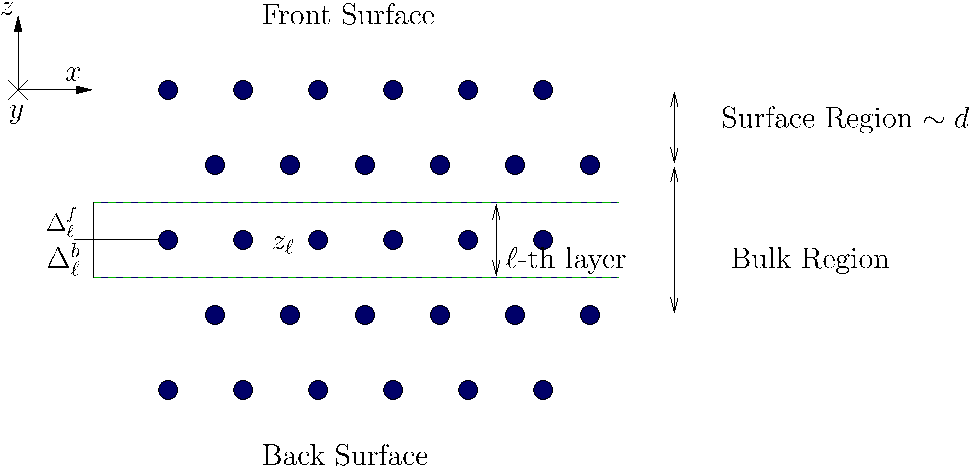
\includegraphics[scale=.7]{content/figures/diag-slab}
\caption{A sketch of the super-cell. The atomic slab corresponds to the circles
representing the atoms of the system.
\label{fslab}} 
\end{figure}

To introduce the cut function ${\boldsymbol{\mathcal{C}}}(z)$ in the calculation
of $\chi^{\mathrm{abc}}$, we start from the operator for the electron current,
$\mathbf{j}(\mathbf{r})=\frac{e}{2}\left(\mathbf{v}^\Sigma |
\mathbf{r}\rangle\langle\mathbf{r} | + | \mathbf{r}\rangle\langle\mathbf{r} |
\mathbf{v}^\Sigma\right)$, that leads to
\begin{equation}
\mathbf{j}^{(N)}(\mathbf{r},t)=\mathrm{Tr}(\mathbf{j}(\mathbf{r})\rho^{(N)}(t))
=
\int \frac{d^3 k}{8\pi^3}
\sum_{nm}
\rho^{(N)}_{nm}(\mathbf{k};t)\mathbf{j}_{mn}(\mathbf{k};\mathbf{r}).
\label{jmic}
\end{equation}
We can derive the $\mathbf{j}_{mn}(\mathbf{k};\mathbf{r})$ matrix elements as
follows. The operator for the electron current is
\begin{equation}\label{hatjmic}
\mathbf{j}(\mathbf{r})
= \frac{e}{2}\left(\mathbf{v}^{\Sigma} |\mathbf{r}\rangle\langle\mathbf{r}|
+ |\mathbf{r}\rangle\langle\mathbf{r}|\mathbf{v}^{\Sigma}\right), 
\end{equation}
where $\mathbf{v}^{\Sigma}$ is the electron's velocity operator to be dealt with
below. We define $\hat{\mu} \equiv |\mathbf{r}\rangle\langle\mathbf{r}|$ and use
the cyclic invariance of the trace to write
\begin{align}\label{jmic2}
\mathrm{Tr}\Big(\mathbf{j}(\mathbf{r})\tilde{\rho}(t)\Big)
&= \mathrm{Tr}\Big(\tilde{\rho}(t)\hat{\mathbf{j}}(\mathbf{r})\Big)\nonumber\\
&= \frac{e}{2}
\left(
  \mathrm{Tr}\Big(\tilde{\rho}\hat{\mathbf{v}}^{\Sigma}\hat{\mu}\Big)
+ \mathrm{Tr}\Big(\tilde{\rho}\hat{\mu}\hat{\mathbf{v}}^{\Sigma}\Big)
\right)\nonumber\\
&= \frac{e}{2}\sum_{n\mathbf{k}}
\left(
\langle n\mathbf{k}|\tilde{\rho}\mathbf{v}^{\Sigma}\hat{\mu}|n\mathbf{k}\rangle
+ \langle n\mathbf{k}|\tilde{\rho}\hat{\mu}\mathbf{v}^{\Sigma}|n\mathbf{k}\rangle
\right)\nonumber\\
&= \frac{e}{2}\sum_{nm}\langle n\mathbf{k}|\tilde{\rho} |m\mathbf{k}\rangle
\left(
  \langle m\mathbf{k}|
  \mathbf{v}^{\Sigma}|\mathbf{r}\rangle
  \langle\mathbf{r}|n\mathbf{k}\rangle
+ \langle m\mathbf{k}|\mathbf{r}\rangle
  \langle\mathbf{r}| \mathbf{v}^{\Sigma} |n\mathbf{k}\rangle
\right)\nonumber\\
\mathbf{j}(\mathbf{r},t)
&= \sum_{nm}\rho_{nm}(\mathbf{k};t)\mathbf{j}_{mn}(\mathbf{k};\mathbf{r}),
\end{align}
where
\begin{equation}\label{jmic3}
\mathbf{j}_{mn}(\mathbf{k};\mathbf{r})=
\frac{e}{2}
\left(
  \langle m\mathbf{k}|\mathbf{v}^{\Sigma} |\mathbf{r}\rangle 
  \langle\mathbf{r}|n\mathbf{k}\rangle
+ \langle m\mathbf{k}|\mathbf{r}\rangle 
  \langle\mathbf{r}|\mathbf{v}^{\Sigma} |n\mathbf{k}\rangle
\right),
\end{equation}
are the matrix elements of the microscopic current operator, and we have used
the fact that the matrix elements between states $|n\mathbf{k}\rangle$ are
diagonal in $\mathbf{k}$, i.e. proportional to $\delta(\mathbf{k}-\mathbf{k}')$.
Integrating the microscopic current $\mathbf{j}(\mathbf{r},t)$ over the entire
slab gives the averaged microscopic current density, $\mathbf{J}(t)$. If we want
the contribution from only one region of the unit cell towards the total
current, we can integrate $\mathbf{j}({\mathbf r},t)$ over the desired region.
Then the contribution to the current density from the chosen region of the slab
is given by
\begin{equation*}
\frac{1}{A}\int d^3r\, \boldsymbol{\mathcal{C}}(z)\, 
\mathbf{J}^{(N)} (\mathbf{r},t)
 \equiv \boldsymbol{\mathcal{J}}^{(N)}(t),
\end{equation*}
where $\boldsymbol{\mathcal{J}}^{(N)}(t)$ is the $N$-th order current
induced in the region specified by $\boldsymbol{\mathcal{C}}(z)$. Therefore we
define
\begin{equation}
e{\boldsymbol{\mathcal{V}}}^{\Sigma}_{mn}(\mathbf{k})
\equiv
\int d^3r\,
\boldsymbol{\mathcal{C}}(z)\,\mathbf{j}_{mn}({\mathbf{k}};\mathbf{r}),
\label{vcal}
\end{equation}
to write the Fourier transform of Eq. \eqref{jmic} as
\begin{equation}
\boldsymbol{\mathcal{J}}^{(N)}(2\omega)=\frac{e}{A}
\int \frac{d^3 k}{8\pi^3}
\sum_{mn}
\boldsymbol{\mathcal{V}}^{\Sigma}_{mn}(\mathbf{k}) 
\rho^{(N)}_{nm}(\mathbf{k};2\omega), 
\label{jmac2}
\end{equation}
that gives the induced microscopic current of the chosen region, to order $N$ in
the external perturbation. From Eqs. \eqref{vcal} and \eqref{jmic3} we obtain
\begin{equation}\label{intj}
{\boldsymbol{\mathcal{V}}}^{\Sigma,\ell}_{mn}({\mathbf k})=
\frac{1}{2}
\int \mathrm{d}^3 r\,
 \mathcal{C}(z)
\bigg[
\langle m\mathbf{k}|\mathbf{v}^\Sigma | \mathbf{r}\rangle
\langle \mathbf{r} | n \mathbf k \rangle +
\langle m\mathbf{k} | \mathbf{r}\rangle
\langle \mathbf{r} | \mathbf{v}^\Sigma | n \mathbf k \rangle\bigg],
\end{equation}  
and using the following property
\begin{align}\label{nl.2}
\langle\mathbf{r}|\mathbf{v}^{\Sigma}(\mathbf{r},\mathbf{r}')|n\mathbf{k}\rangle
&= \int d^3 r'' 
\langle\mathbf{r}|
\mathbf{v}^{\Sigma}(\mathbf{r},\mathbf{r}')
|\mathbf{r}''\rangle
\langle\mathbf{r}''|n\mathbf{k}\rangle\nonumber\\
&= \mathbf{v}^{\Sigma}(\mathbf{r},\mathbf{r}'')
\int d^3 r'' \langle\mathbf{r}|\mathbf{r}''\rangle
\langle\mathbf{r}''|n\mathbf{k}\rangle\nonumber\\
&= \mathbf{v}^{\Sigma}(\mathbf{r},\mathbf{r}')
\psi_{n\mathbf{k}}(\mathbf{r}),
\end{align}
that stems from the fact that the operator
$\mathbf{v}^\Sigma(\mathbf{r},\mathbf{r}')$ does not act on $\mathbf{r}''$, we
can write
\begin{align}\label{nl.3}
\boldsymbol{\mathcal{V}}^{\Sigma,\ell}_{mn}({\mathbf k})
&=
\frac{1}{2}
\int 
 \boldsymbol{\mathcal{C}}(z)
 \bigg[
\psi_{n\mathbf{k}}(\mathbf{r})
\mathbf{v}^{\Sigma *}\psi^{*}_{m\mathbf{k}}(\mathbf{r})
+ 
\psi^*_{m\mathbf{k}}(\mathbf{r})\mathbf{v}^{\Sigma}
\psi_{n\mathbf{k}}(\mathbf{r})
\bigg]\,\mathrm{d}^3 r
\nonumber\\
&=
\int 
\psi^*_{m\mathbf{k}}(\mathbf{r})
\left[\frac{\boldsymbol{\mathcal{C}}(z) \mathbf{v}^\Sigma +
\mathbf{v}^\Sigma \boldsymbol{\mathcal{C}}(z)}{2}\right]
\psi_{n\mathbf{k}}(\mathbf{r})\,\mathrm{d}^3 r
\nonumber\\
&=
\int 
\psi^*_{m\mathbf{k}}(\mathbf{r})
\boldsymbol{\mathcal{V}}^{\Sigma}
\psi_{n\mathbf{k}}(\mathbf{r})\,\mathrm{d}^3 r
,
\end{align}
where we used the hermitian property of $\mathbf{v}^\Sigma$ and defined
\begin{align}\label{nl.4}
\boldsymbol{\mathcal{V}}^{\Sigma}
= \frac{\boldsymbol{\mathcal{C}}(z) \mathbf{v}^\Sigma
+ \mathbf{v}^\Sigma \boldsymbol{\mathcal{C}}(z)}{2},
\end{align} 
We see that the replacement
\begin{equation}
\mathbf{V} \to \boldsymbol{\mathcal{V}}
= \frac{\boldsymbol{\mathcal{C}}(z) \mathbf{V}
+ \mathbf{V} \boldsymbol{\mathcal{C}}(z)}{2},
\label{vcali}
\end{equation} 
is all that is needed to change any of the electron velocity operators
$\mathbf{V}$ to the new velocity operator $\boldsymbol{\mathcal{V}}$ that
implicitly takes into account the contribution of the region of the slab given
by $\boldsymbol{\mathcal{C}}(z)$. We note that this modified operator is
hermitian as it should.\cite{note2} The operator $\mathbf{V}$ could be any of
those given by Eq. \eqref{vop2}, thus
\begin{align}\label{vopii}
\boldsymbol{\mathcal{V}}^{\Sigma}
&= \boldsymbol{\mathcal{V}}^{\mathrm{LDA}}
+ \boldsymbol{\mathcal{V}}^{S}\nonumber\\
\boldsymbol{\mathcal{V}}^{\mathrm{LDA}} 
&= \boldsymbol{\mathcal{V}}
+ \boldsymbol{\mathcal{V}}^{\mathrm{nl}}.
\end{align}
As shown in Appendix \ref{app:voila}, Eq. \eqref{chon.8} is generalized to
$\boldsymbol{\mathcal{V}}^{\Sigma}_{nm} =
(\omega^\Sigma_{nm}/\omega^{\mathrm{LDA}}_{nm})
\boldsymbol{\mathcal{V}}^{\mathrm{LDA}}_{nm}$ from which
$\boldsymbol{\mathcal{V}}^{\Sigma}_{nm}$ can be readily calculated. As a
consistency test we have calculated the matrix elements of
$\boldsymbol{\mathcal{V}}^{\mathrm{LDA}}$ and
$\boldsymbol{\mathcal{V}}^{\mathcal{S}}$ separately, according to the derivation
presented in Appendix \ref{app:calvs} and \ref{app:calpcalc}, and confirm that
both approaches yield identical results for
$\chi^{\mathrm{abc}}_{\mathrm{surface}}$. If not stated differently,
calligraphic letters correspond to layer quantities.

To limit the SHG response to one surface, Eq. \eqref{vcali} for
$\boldsymbol{\mathcal{V}}$ was proposed in Ref. \cite{reiningPRB94} and later
used in Refs. \cite{mendozaPRL98}, \cite{mendozaPRB01}, \cite{sanoPRB02}, and
\cite{mejiaRMF04} also in the context of SHG. The layer-by-layer analysis of
Refs. \cite{hoganPRB03} and \cite{castilloPRB03} used Eq. \eqref{sz}, limiting
the current response to a particular layer of the slab and used to obtain the
anisotropic linear optical response of semiconductor surfaces. However, the
first formal derivation of this scheme is presented in Ref. \cite{mendozaPRB06}
for the linear response. In this thesis I formally introduce the cut function
$\boldsymbol{\mathcal{C}}(z)$ for the second-harmonic optical response of
semiconductor surfaces, from an average of the second order polarization over
the region of interest.


%%%%%%%%%%%%%%%%%%%%%%%%%%%%%%%%%%%%%%%%%%%%%%%%%%%%%%%%%%%%%%%%%%%%%%%%%%%%%%%%
%%%%%%%%%%%%%%%%%%%%%%%%%%%%%%%%%%%%%%%%%%%%%%%%%%%%%%%%%%%%%%%%%%%%%%%%%%%%%%%%

\section{Microscopic surface susceptibility}

In this section we obtain the expressions for the surface susceptibility tensor
$\chi^{\mathrm{abc}}_{\mathrm{surface}}$. Using
$\boldsymbol{\mathcal{J}}=d\boldsymbol{\mathcal{P}}/dt$ and Eq. \eqref{jmac2} we
obtain the SH polarization of a given region as
\begin{equation}\label{Pjikn}
\boldsymbol{\mathcal{P}}^{(2)}(2\omega)
= \frac{ie}{2A\tilde\omega} \int \frac{d^3 k}{8\pi^3}
\sum_{mn} \boldsymbol{\mathcal{V}}^{\Sigma}_{mn}(\mathbf{k})
\rho^{(2)}_{nm}(\mathbf{k};2\omega),
\end{equation}
and using Eqs. \eqref{pshg} and \eqref{rtilde33} leads to
\begin{align}\label{Pjikn2}
\chi^{\mathrm{a}\mathrm{b}\mathrm{c}}(-2\omega;\omega,\omega) 
&= \frac{e^2}{2A\hbar\tilde\omega}
\int \frac{d^3 k}{8\pi^3}
\sum_{mn}
\frac{\boldsymbol{\mathcal{V}}^{\Sigma,\mathrm{a}}_{mn}(\mathbf{k})}
{\omega^\Sigma_{nm\mathbf{k}}-2\tilde\omega}
\bigg[
i\sum_q\left(r_{nq}^{\mathrm{b}}B_{qm}^{\mathrm{c}}(\mathbf{k},\omega) -
  B_{nq}^{\mathrm{c}}(\mathbf{k},\omega) 
  r_{qm}^{\mathrm{b}}\right)\nonumber\\
&\qquad\qquad\qquad\qquad\qquad\qquad\qquad\qquad\qquad\qquad\qquad\quad
-\Big(B_{nm}^{\mathrm{c}}(\mathbf{k},\omega)\Big)_{;k^{\mathrm{b}}}
\bigg],
\end{align}
which gives the susceptibility
$\chi^{\mathrm{a}\mathrm{b}\mathrm{c}}(-2\omega;\omega,\omega)$ of the layers of
the slab specified by $\boldsymbol{\mathcal{C}}(z)$. We mention that the units
of $\chi^{\mathrm{a}\mathrm{b}\mathrm{c}}(-2\omega;\omega,\omega)$ are m$^2$/V,
as they should be for a surface SH susceptibility. Using Eq. \eqref{rho1} we
split this equation into two contributions from the first and second terms on
the right hand side of Eq. \eqref{Pjikn2}:
\begin{equation}
\chi^{\mathrm{a}\mathrm{b}\mathrm{c}}_i (-2\omega;\omega,\omega)
=-\frac{e^3}{A\hbar^22\tilde\omega}
\int \frac{d^3 k}{8\pi^3}
\sum_{mn}
\frac{\boldsymbol{\mathcal{V}}_{mn}^{\Sigma,\mathrm{a}}}
{\omega^\Sigma_{nm}-2\tilde\omega}
\left(\frac{f_{mn}r_{nm}^{\mathrm{b}}}
{\omega^\Sigma_{nm}-\tilde\omega}\right)_{;k^{\mathrm{c}}},
\label{chii}
\end{equation} 
related to intraband transitions, and 
\begin{equation}
\chi^{\mathrm{a}\mathrm{b}\mathrm{c}}_e (-2\omega;\omega,\omega)
=\frac{ie^3}{A\hbar^22\tilde\omega}
\int \frac{d^3 k}{8\pi^3}
\sum_{qmn}
\frac{\boldsymbol{\mathcal{V}}_{mn}^{\Sigma,\mathrm{a}}}{\omega^\Sigma_{nm}-2\tilde\omega}
\left(
\frac{r_{nq}^{\mathrm{c}} r_{qm}^{\mathrm{b}} 
f_{mq}}{\omega^\Sigma_{qm}-\tilde\omega}
-\frac{r_{nq}^{\mathrm{b}} r_{qm}^{\mathrm{c}} 
f_{qn}}{\omega^\Sigma_{nq}-\tilde\omega}
\right),
\label{chie}
\end{equation} 
related to interband transitions. The generalized derivative in Eq. \eqref{chii}
is dealt with by the chain rule
\begin{equation}
\left(\frac{f_{mn}r_{nm}^{\mathrm{b}}}
{\omega^\Sigma_{nm}-\tilde\omega}\right)_{;k^{\mathrm{c}}}=
\frac{f_{mn}}{\omega^\Sigma_{nm}-\tilde\omega}
\left(r_{nm}^\mathrm{b}\right)_{;k^{\mathrm{c}}}
-\frac{f_{mn}r_{nm}^{\mathrm{b}}\Delta_{nm}^\mathrm{c}}
{(\omega^\Sigma_{nm}-\tilde\omega)^2},
\label{gene2}
\end{equation}
where substituting $H^\Sigma_0$ into Eq. \eqref{conmri3n} and then Eq.
\eqref{chon.10} we obtain
\begin{equation}\label{eli.13}
\left(\omega^\Sigma_{nm}\right)_{;k^{\mathrm{a}}}
= \left(\omega^\mathrm{LDA}_{nm}\right)_{;k^{\mathrm{a}}}
= v_{nn}^{\mathrm{LDA},\mathrm{a}}
- v_{mm}^{\mathrm{LDA},\mathrm{a}}\equiv\Delta_{nm}^{\mathrm{a}}.
\end{equation} 
The apparent divergence as $\tilde\omega\to 0$ in Eqs. \eqref{chii} and
\eqref{chie}, is removed  by a partial fraction expansion over $\tilde\omega$.
Using time-reversal symmetry, an integration by parts to remove the square in
the denominator of the second term of Eq. \eqref{gene2}, and taking the limit of
$\eta\to 0$, we obtain the following expressions for the imaginary parts of Eqs.
\eqref{chii} and \eqref{chie},
\begin{subequations}\label{eq:chis}
\begin{equation}
\mathrm{Im}[\chi^{\mathrm{a}\mathrm{b}\mathrm{c}}_{e,\omega}]= 
\frac{\pi |e|^3}{2\hbar^2}
\int \frac{d^3 k}{8\pi^3}
\sum_{vc}\sum_{q\neq(v,c)}\frac{1}{\omega^\Sigma_{cv}}
\left[
\frac{\mathrm{Im}[\mathcal{V}^{\Sigma,\mathrm{a}}_{qc}
\{r^{\mathrm{b}}_{cv}r^{\mathrm{c}}_{vq}\}]}
{(2\omega^\Sigma_{cv}-\omega^\Sigma_{cq})} 
-\frac{\mathrm{Im}[\mathcal{V}^{\Sigma,\mathrm{a}}_{vq}
\{r^{\mathrm{c}}_{qc}r^{\mathrm{b}}_{cv}\}]}
{(2\omega^\Sigma_{cv}-\omega^\Sigma_{qv})}
\right]\delta(\omega^\Sigma_{cv}-\omega),
\end{equation}  
\begin{equation}
\mathrm{Im}[\chi^{\mathrm{a}\mathrm{b}\mathrm{c}}_{i,\omega}]= 
\frac{\pi\vert e\vert^3}{2\hbar^2}
\int \frac{d^3 k}{8\pi^3}
\sum_{cv}\frac{1}{(\omega^\Sigma_{cv})^{2}}
\left[
\mathrm{Re}\left[\left\{r^{\mathrm{b}}_{cv}
\left(\mathcal{V}^{\Sigma,\mathrm{a}}_{vc}\right)_{;k^{\mathrm{c}}}\right\}
\right]
+\frac{\mathrm{Re}\left[\mathcal{V}^{\Sigma,\mathrm{a}}_{vc}
\left\{r^{\mathrm{b}}_{cv}\Delta^{\mathrm{c}}_{cv}\right\}
\right]}{\omega^\Sigma_{cv}} 
\right]\delta(\omega^\Sigma_{cv}-\omega),
\end{equation}
\begin{equation}
\mathrm{Im}[\chi^{\mathrm{a}\mathrm{b}\mathrm{c}}_{e,2\omega}]= 
-\frac{\pi |e|^3}{2\hbar^2}
\int \frac{d^3 k}{8\pi^3}
\sum_{vc}\frac{4}{\omega^\Sigma_{cv}}
\left[
\sum_{v'\ne
  v}\frac{\mathrm{Im}[\mathcal{V}^{\Sigma,\mathrm{a}}_{vc}
  \{r^{\mathrm{b}}_{cv'}r^{\mathrm{c}}_{v'v}\}]}
{2\omega^\Sigma_{cv'}-\omega^\Sigma_{cv}}
- \sum_{c'\ne
  c}\frac{\mathrm{Im}[\mathcal{V}^{\Sigma,\mathrm{a}}_{vc}
  \{r^{\mathrm{c}}_{cc'}r^{\mathrm{b}}_{c'v}\}]}
{2\omega^\Sigma_{c'v}-\omega^\Sigma_{cv}}
\right]\delta(\omega^\Sigma_{cv}-2\omega),
\end{equation}
\begin{equation}
\mathrm{Im}[\chi^{\mathrm{a}\mathrm{b}\mathrm{c}}_{i,2\omega}]= 
 \frac{\pi \vert
   e\vert^{3}}{2\hbar^2}
\int \frac{d^3 k}{8\pi^3}
\sum_{vc}\frac{4}{(\omega^\Sigma_{cv})^{2}}
\left[\mathrm{Re}\left[\mathcal{V}^{\Sigma,\mathrm{a}}_{vc}
\left\{\left(r^{\mathrm{b}}_{cv}\right)_{;k^{\mathrm{c}}}
\right\}\right] -
\frac{2\mathrm{Re}\left[\mathcal{V}^{\Sigma,\mathrm{a}}_{vc}
\left\{r^{\mathrm{b}}_{cv}\Delta^{\mathrm{c}}_{cv}\right\}\right]}
{\omega^\Sigma_{cv}}\right]\delta(\omega^\Sigma_{cv}-2\omega),
\end{equation}
\end{subequations}
where we have split the interband and intraband $1\omega$ and $2\omega$
contributions and suppressed the $\omega$ arguments for convenience of notation.
The factor of 2 for spin degeneracy is not included in Eq. \eqref{eq:chis}. The
real part of each contribution can be obtained through a Kramers-Kronig
transformation\cite{nicolasPRB14} and $\chi^{\mathrm{a}\mathrm{b}\mathrm{c}}=
\chi^{\mathrm{a}\mathrm{b}\mathrm{c}}_{e,\omega} 
+\chi^{\mathrm{a}\mathrm{b}\mathrm{c}}_{e,2\omega}
+\chi^{\mathrm{a}\mathrm{b}\mathrm{c}}_{i,\omega} 
+\chi^{\mathrm{a}\mathrm{b}\mathrm{c}}_{i,2\omega}
$.
To fulfill the required intrinsic permutation symmetry, the $\{\}$ notation
symmetrizes the $\mathrm{b}\mathrm{c}$ Cartesian indices, i.e. $\{u^{\mathrm{b}}
s^{\mathrm{c}}\}=(u^{\mathrm{b}}s^{\mathrm{c}}+u^{\mathrm{c}}s^{\mathrm{b}})/2$,
and thus $\chi^{\mathrm{a}\mathrm{b}\mathrm{c}}=\chi^{\mathrm{acb}}$. The full
expressions for $\chi^{\mathrm{a}\mathrm{b}\mathrm{c}}(-2\omega;\omega,\omega)$,
along with the various quantities involved in Eq. \eqref{eq:chis} are given in
the Appendix \ref{appv}. We mention that if we take
$\boldsymbol{\mathcal{C}}(z)=1$ through out, the layered matrix elements
$\boldsymbol{\mathcal{V}}^{\Sigma}_{nm}$ become standard bulk-like
$\mathbf{v}^{\Sigma}_{nm}$ matrix elements. We mention that in this case, Eq.
\eqref{eq:chis} is equivalent to the expressions of Ref. \cite{cabellosPRB09},
valid for bulk semiconductors. Finally, we could also calculate the nonlinear
surface susceptibility as
\begin{equation}
\boldsymbol{\chi}_{\mathrm{surface}}(-2\omega;\omega,\omega)
= \sum_{\{\ell\}}\boldsymbol{\chi}^\ell(-2\omega;\omega,\omega),
\label{chiijksur}
\end{equation} 
where $\ell$ would denote a particular layer chosen through
$\boldsymbol{\mathcal{C}}^\ell(z)$ of Eq. \eqref{sz} and $\{\ell\}$ is meant to
be a chosen set of layers. For instance, one can take a single layer
encompassing half of the slab, or take each atomic layer individually to the
middle of the slab. For the first case there is a single summand in Eq.
\eqref{chiijksur}. For the second case there is a sum from $\ell=1$, denoting
the first layer right at the surface, to $\ell=N$, denoting the layer at the
middle of the slab that behaves like a bulk layer. We remark that the value of
$N$ is not universal and the slab needs to have enough atomic layers in order to
give converged results for
$\boldsymbol{\chi}_{\mathrm{surface}}(-2\omega;\omega,\omega)$. We can use Eq.
\eqref{chiijksur} for either the front or the back surface.

In Appendices \ref{app:gdernl} and \ref{app:calvs} we demonstrate how to
calculate the generalized derivatives of
$\left(\mathbf{r}_{nm}\right)_{;\mathbf{k}}$ and
$\left(\mathcal{V}^{\Sigma,\mathrm{a}}_{nm}\right)_{;\mathbf{k}}$. From
Appendix \ref{app:gdernl} we find that
$T_{nm}^{\mathrm{ab}}$, given by
\begin{align}\label{tau.1}
T_{nm}^{\mathrm{ab}}
= \frac{\hbar}{m_{e}}\delta_{ab}\delta_{nm}
- \hbar L_{nm}^{\mathrm{ab}},
\end{align}  
where
\begin{align}\label{tau.2}
L_{nm}^{\mathrm{ab}}
= \frac{i}{\hbar}\left[r^{\mathrm{b}},v^{\mathrm{nl},\mathrm{a}}\right]_{nm},
\end{align}
is the contribution to the generalized derivatives
$\left(\mathbf{r}_{nm}\right)_{;\mathbf{k}}$, and
$\left(\mathcal{V}^{\Sigma,\mathrm{a},\ell}_{nm}\right)_{;\mathbf{k}}$ coming
from the nonlocal part of the pseudopotential, $\mathbf{v}^{\mathrm{nl}}$. In
Appendix \ref{app:calt} we calculate $L^{\mathrm{ab}}_{nm}$. It is shown in Ref.
\cite{valerie} that this term has a very small numerical value, and a
computational time of at least an order of magnitude larger than for all the
other terms involved in the expressions for $\chi^{\mathrm{abc}}$. Therefore, we
neglect it throughout this thesis and take
\begin{align}\label{tau.69}
T_{nm}^{\mathrm{ab}} \approx \frac{\hbar}{m_{e}}\delta_{ab}\delta_{nm}.
\end{align} 


%%%%%%%%%%%%%%%%%%%%%%%%%%%%%%%%%%%%%%%%%%%%%%%%%%%%%%%%%%%%%%%%%%%%%%%%%%%%%%%%
%%%%%%%%%%%%%%%%%%%%%%%%%%%%%%%%%%%%%%%%%%%%%%%%%%%%%%%%%%%%%%%%%%%%%%%%%%%%%%%%

\section{About the code}

The TINIBA code is a suite of scripts that work with the popular ABINIT package
to run and calculate optical properties of crystalline semiconductors by
parallelizing the computation of the different quantities involved in the
procedure. I have created a
\href{https://github.com/roguephysicist/tiniba-manual}{Github repository}
with the user manual for the TINIBA code, along with a detailed manuscript on
how we coded the expressions derived in this chapter.


%%%%%%%%%%%%%%%%%%%%%%%%%%%%%%%%%%%%%%%%%%%%%%%%%%%%%%%%%%%%%%%%%%%%%%%%%%%%%%%%
%%%%%%%%%%%%%%%%%%%%%%%%%%%%%%%%%%%%%%%%%%%%%%%%%%%%%%%%%%%%%%%%%%%%%%%%%%%%%%%%

\section{Conclusions}

I have presented a formulation to calculate the surface second-harmonic (SSH)
susceptibility tensor
$\boldsymbol{\chi}_{\mathrm{surface}}(-2\omega;\omega,\omega)$, using the length
gauge formalism and within the independent particle approximation (IPA). It
includes on equal footing: (i) the scissors correction, (ii) the contribution of
the non-local part of the pseudopotentials, and (iii) the cut function. We have
neglected local field and excitonic effects. Although these are important
factors in the optical response of a semiconductor, their efficient calculation
is theoretically and numerically challenging and still under debate
\cite{beyond}. This merits further study but is beyond the scope of this thesis.
Nevertheless, the inclusion of aforementioned contributions in our scheme opens
the unprecedented possibility to study surface SHG with more versatility and
more accurate results.


\stopcontents[chapters]

